\documentclass[a4paper,12pt]{report}
\usepackage{algorithmic}
\usepackage[linesnumbered,ruled,vlined]{algorithm2e}
\usepackage[margin=2cm]{geometry}
\usepackage[utf8]{inputenc}
\usepackage{listings} 
\usepackage{graphicx} 
\usepackage{color}
\usepackage[dvipsnames]{xcolor}
\usepackage{hyperref}
\usepackage{mdframed}
\usepackage{fancyvrb}
\usepackage{cite}

\newcommand{\currentdata}{14 February 2015}
\newtheorem{example}{Example}

\begin{document}
\vspace{-5cm}
\begin{center}
Department of Computer Science\\
Technical University of Cluj-Napoca\\

\includegraphics[width=10cm]{fig/footer}
\end{center}
\vspace{1cm}
\begin{center}
\begin{Large}
 \textbf{Introduction to Artificial Intelligence}\\
\end{Large}
\textit{Laboratory activity 2016-2017}\\
\vspace{3cm}
Name: Veres Adela\\
Group: 30235\\
Email: adela.veres@yahoo.ro\\
\vspace{12cm}
Assoc. Prof. dr. eng. Adrian Groza\\
Adrian.Groza@cs.utcluj.ro\\
\vspace{1cm}

\includegraphics[width=10cm]{fig/footer}
\end{center}

\tableofcontents


\chapter{Installing the tool ($W_2$)}
\vspace{0.5cm}

%List the performed steps required to run the tool. 
The steps for installation are:

  -Download and install gcc (only if not available in our unix/linux distribution).
  
  -Download and install lparse.
\begin{enumerate}
 \item Download lparse-1.1.2 source package.
 \item Type "cd" in the terminal, to change to the directory containing lparse source code and type "./configure" to configure lparse for the system.

 ./configure
\item Type "make" to compile the binaries.

make
\item Type "make install" to install lparse.

make install
\item If we want to remove the object files from the source code directory we may type "make clean" to do it.

make clean
\end{enumerate}

  By default, lparse is installed to the directory /usr/local/bin. We may change the directory by giving the "configure" option the option "- -prefix=path".

  -Download and install smodels.
\begin{enumerate}
 \item Download smodels-2.34 source package.
 \item In the terminal, change to the directory containing the source code.
 \item Type "make", to compile the binaries. It will output the "smodels" executable file.
 \item Move the "smodels" file to /usr/bin/.
\end{enumerate}

  -Download and install the SWI-Prolog interpreter from: http://www.swi-prolog.org/Download.html.

  
  -Download and uncompress the file fal-1.0.tar.gz in a separate directory, from: http://www.dc.fi.udc.es/~cabalar/fal/falf-1.0.tar.gz

  Then run 'make' in the created directory.
  In order to do this, type the following commands in the terminal:
\begin{verbatim}
$ gunzip fal-1.0.tar-gz
$ tar -xvf fal-1.0.tar
$ cd falf-1.0
$ make
\end{verbatim}

Now, the 'falf' and 'getterms' executables should be present in the falf-1.0 directory.

In order to make them accessible, make a copy of each of them in some directory in your PATH (for instance, /usr/local/bin).

 
 
The tool was installed on:
\begin{verbatim}
Fedora 20 (Heisenbug), x86_64
Java 1.8.0_73

\end{verbatim}

Running the tool
\begin{verbatim}
Fedora 20 (Heisenbug), x86_64
Java 1.8.0_73

\end{verbatim}



\chapter{Running and understanding examples ($W_3$)}

	Examples are located in a directory named likewise: "examples", which cand be found in the "falf-1.0" directory previously dealt with.
In order to run an example, first open a terminal and type "falf", in order to start the program's frontend.
A small presentation of falf, including a list with special commands that cand be used should appear, as shown in the following capture:

\vspace{0.5cm}
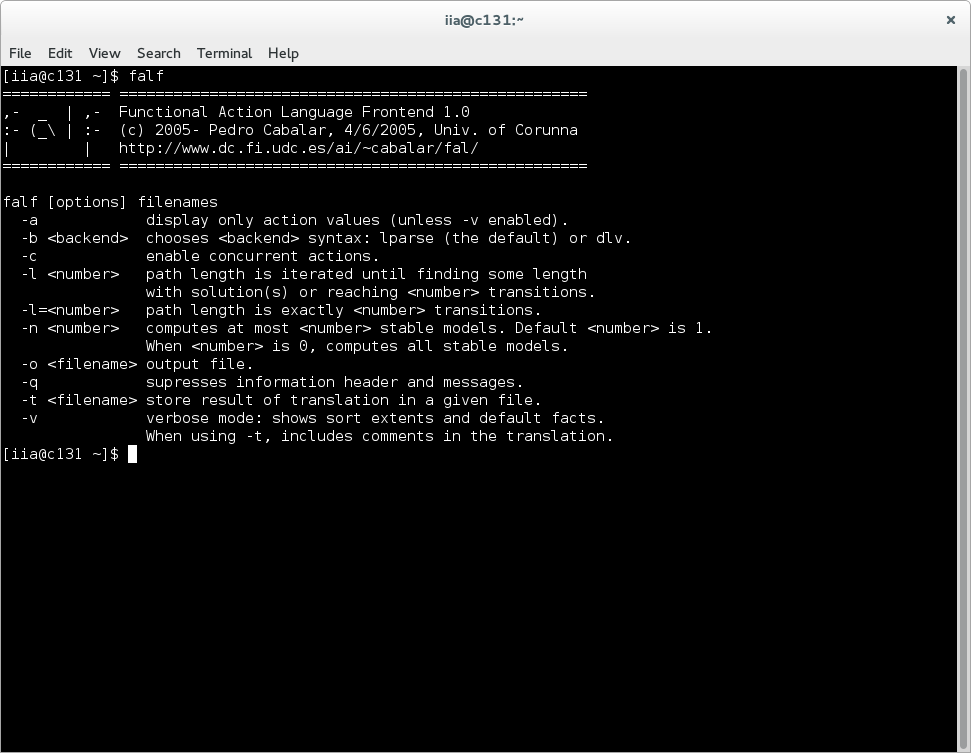
\includegraphics[scale=0.4]{Screenshot_terminal_Falf.png}

\section {Fibonacci Numbers}
 
	The Fibonacci Sequence is a series of numbers, where the next number is found by adding up the two numbers before it.
 We are going to run an example from the "examples" directory, the 'fibo.fal', which computes the first ten values of the Fibonacci Numbers.
	The example should output the following result:
 \begin{verbatim}
  fib(1) = 1
  fib(2) = 1
  fib(3) = 2
  fib(4) = 3
  fib(5) = 5
  fib(6) = 8
  fib(7) = 13
  fib(8) = 21
  fib(9) = 34
  fib(10) = 55
 \end{verbatim}

	 In order to run the example, first make sure to be located in the "examples" directory.
 Now you must create a temporal file, in order for the executable program to use it.
	To achieve this, type the following from the terminal:
 \begin{verbatim}
  >fibo.fal.tmp
 \end{verbatim}
	To actually run the program, type in:
 \begin{verbatim}
  falf fibo.fal
 \end{verbatim}
	Try using option -v (verbose mode) to print the extent of all sorts:
\begin{verbatim}
falf -v examples/fibo.fal
\end{verbatim}
	At this point, the console should print the expected result, the first ten values of the Fibonnaci series, as listed above.


	In an ordinary text file we write our code and save it with the extension ".fal". As in the case of the "fibo.fal" file, this contains the main code for our program to run. 

	We will now examine the structure of the file. Here is the content of the file:
\begin{verbatim}  
instances
	int 1..100.
	index 1..8.

static
	fib : index -> int.

rules
	fib(1) = 1.
	fib(2) = 1.
	fib(X+2) = fib(X) + fib(X+1) :- vars X: index.

\end{verbatim}

	The \textit{fib} function is defined using the \textit{static} word, which means that a set of function definitions follows. In fact the term \textit{static} further specifies that all the values of the functions below \textbf{will not vary} along time. We will see later that we can deal with transition systems and that other types of functions may change along time. A function declaration is done following the usual mathematical notation.


\begin{addmargin}
$\langle function\_name\rangle : \langle set1\rangle \times \langle set2\rangle \times ... \times \langle setN\rangle   \rightarrow   \langle range\rangle$ .
\end{addmargin}


	In this case, function \textit{fib} takes just one argument from a sort called \textit{index} and returns a value from sort \textit{int}. The instances of these two sorts are declared as shown above, in the \textit{instances} block, meaning that \textit{index} is a number varying from 1 to 8, and \text{int} a number from 1 to 100.
The ordering among FAL sentences is irrelevant: you can declare functions referring to sorts that occur below in the code, or even in a different file. There exists a predefined sort called \textit{boolean}, whose instances are \texit{true} and \textit{false}, as expected. When a function  \textit{f(X)} has a \textit{boolean} range (i.e., it is a predicate) we allow the abbreviation of \textit{f(X)=true} just as \textit{f(X)} and the abbreviation of \textit{f(X)=false} as \textit{not f(X)}.

	When declaring functions or sorts, we can also refer to set expressions. For instance, function \textit{fib} could also be defined as:

\begin{verbatim}
static 
fib : {1..8} -> {1..100}.
\end{verbatim}
	
	An extensional set is represented as a list of elements separated by commas and between braces, like, for instance, 
\begin{verbatim}
{red, blue, green}.
\end{verbatim}
As we can see, the notation . . is used for comprising an interval of integer values. Another example of extensional set could be: 
\begin{verbatim}
{1, 3, 5..10, null}.
\end{verbatim}
	Set union, intersection and difference are respectively represented by operators '+', '*' and '-'.
	The \textit{rules} block, in the code above expresses the functionality of \textit{fib}. The first two values of \textit{fib} are known (1), and the following are computed by adding the previous two values.
 

\chapter{Understanding conceptual instrumentation ($W_4$)}
	
	
	The Functional Action Language (FAL) is thought for describing constraint satisfaction problems that may involve temporal reasoning about actions and change.
A problem is expressed in terms of a set of functions and a set of rules that establish the relation among values for those functions.
Each solution to the problem is a possible assigment of function values that "agrees" with the set of rules.

	Syntactically, FAL is very close to languages from Functional Logic Programming. Rules have a Prolog-style form like, for instance:
\begin{verbatim}
  mother(X,Y) :- parent(X,Y), female(Y).
\end{verbatim}

	This is to be read as: "Y is X's mother if Y is one of X's parents and Y is female".
As in Prolog, identifiers beginning with a capital letter, like X or Y, represent variables.
The main difference with respect to Prolog is the posibility of referring to funcion values in place of predicate atoms.
As an example, since there (usually) exists a unique mother, we could represent mother(X) as a function, rather than as a binary predicate:
\begin{verbatim}
  mother(X)=Y :- parent(X,Y), female(Y).
\end{verbatim}

	But the most interesting advantage of using functions is, of course, that they can be nested as arguments of other functions or expressions.
As an example, consider the rule:
\begin{verbatim}
  grandmother(X,mother(Y)):- parent(X,Y).
\end{verbatim}
meaning that the grandmother of X is the mother of any of X's parents.
	
	As shown in the previous chapter, a basic structure of a FAL program will usually include the blocks: \textit{instances} -used for instantiating variables-, \textit{static} - used for defining functions - and \textit{rules} - in order to specify the logical flow of the function.

\section{Variables}

	In the Fibonnaci example, a local variable $\times$ of type \textit{index} is used in the third rule of the example. All FAL variables must be declared with a given range. There are two ways of declaring a variable: as a \textit{local} or as a \textit{global} variable. A rule may include several declarations of \textit{local} variables following the next pattern:

$ \langle head \rangle :- \langle body \rangle  vars \langle vardecls \rangle $.

	The term $\langle vardecls \rangle $ refers to a set of variable declarations separated by commas. When $\langle vardecls \rangle $ is empty, we remove the tag \textit{vars}. Furthermore, if $\langle body \rangle $ is also empty, we remove the condtional operator ":-" too, and the rule (i.e., the head alone) is called a \textbf{\textit{fact}}.

Each variable declaration has the shape:

$\langle varname \rangle  : \langle range \rangle $ .

As an example of declaration of local variables we could have:
\begin{verbatim}
mother(X)=Y: parent(X,Y), female(Y) vars X : person, Y : person.
\end{verbatim}


As a shorthand, when declaring several variables with the same range, we can group them as follows:
\begin{verbatim}
mother(X)=Y: parent(X,Y), female(Y) vars X, Y : person.
\end{verbatim}

A second type of variable declaration is the use of a \textit{global} variable. This is done by including a \textit{vars} clause, but externally to any rule, like for instance:
\begin{verbatim}
vars
X, Y : person.

rules
mother(X)=Y :- parent(X,Y), female(Y).
\end{verbatim}

This is sometimes more comfortable, as it avoids repeating the variable range in all the rules it is used. When there exists a coincidence in the names of a global and a local variable, the former is hidden by the latter, as expected.

\section{Default Values}

One of the particular features of FAL functions is that they allow the definition of a default value. As an example, consider the following pair of definitions of \textit{boolean} functions (or just predicates):

\begin{addmargin}
$likes: person \times  person \rightarrow boolean.$

$parent: person \times person \rightarrow boolean = false.$
\end{addmargin}

The first predicate has no default value and so, we may declare that \textit{likes(X,Y)} is \textit{true} or assert instead that it is \textit{false}, but when we do not provide any information, it will have \textit{no defined value}. When this happens, we say that \textit{likes(X,Y)} is just \textbf{unknown}: in fact, we can use the boolean expression \textbf{unknown(likes(X,Y))} (or its negation) in the body of any FAL rule. The second predicate, \textit{parent}, has been defined as \textit{false} by default. This means that when no evidence about \textit{parent(X,Y)} is provided, we will \textbf{assume by default} that \textit{Y} is not one of \textit{X}'s parents. Note that this is important, since we usually want to avoid describing all the people who \textit{are not} parents of a given person.

\section{Functional Answer Sets}
In order to understand how default values work, consider by now that FAL rules had the simplified syntax:

\begin{addmargin}
$g=v :- f_1=v_1 , f_2=v_2 , ..., f_n=v_n. $ (1)
\end{addmargin}

where $g$ and all the $f_i$ are functions whereas $v$ and the $v_j$ are values. Any FAL program can be translated into a set of rules of this form by a \textbf{grounding} process: essentially, we remove variables and nested function references, replacing them by their possible values. A set of rules like (1) is called a\textit{ ground FAL program}.


An {\color{orange} interpretation} is a (possibly partial) mapping that assigns to each function $f$ one value from its declared range, or perhaps no value at all, leaving $f$ undefined or unknown. Of course, the latter may only happen when function $f$ has no defined default value. The interpretation can be represented as a set of pairs $(f=v)$ with at most one pair per each function $f$. An interpretation \textit{I} is said to be a {\color{orange}model} of a ground FAL program when all rules like (1) in the program satisfy that $(g=v)$ belongs to\textit{I} if all the body pairs $(f_1=v_1), ..., (f_n=v_n)$ belong to I. Given an interpretation \textit{I} , we call {\color{orange}\textit{default(I)}} to the set of pairs $(f=v)$ in \textit{I} for which $v$ is the default value of $f$. An interpretation \textit{I} is a {\color{orange}functional answer set} of a ground FAL program \textit{P} when \textit{I} is a minimal model of the augmented program: \textit{P} U \textit{default(I)}.

In other words, we first guess some arbitrary possible model \textit{I} for the program P. Then we add to P all the facts in \textit{I} that correspond to default value assignments. Finally, getting the minimal model of this augmented program \textit{P} U \textit{default(I)} informally corresponds to an exhaustive application of its rules until no new fact is obtained. If, as a result of this process, we get back the original assumption I, then we have obtained a functional answer set.


Example: consider the following ground FAL program:


\begin{verbatim}
static 
f, g, h : {0..10} = 0.

rules
f=7 :- g=0.
g=3 :- f=0.
h=5 :- g=3, f=0.
\end{verbatim}

Take the interpretation \textit{I} = $\{f=0, g=3, h=5\}$. The default portion of I is \textit{default(I)} = $\{f=0\}$, since it is the only assigment of a default value. Now we apply the second rule knowing $\{f=0\}$ to get g=3. But as we have now $\{f=0, g=3\}$ we apply the third rule to get $h=5$. As we cannot apply more rules, the final result of this process is $\{f=0, g=3, h=5\}$ which coincides with the original $I$, and so, becomes a functional answer set. You can similarly check that this program actually has a second (functional) answer set: $\{f=7, g=0, h=0\}$. 
\vspace{0.5cm}
\begin{mdframed}[backgroundcolor=blue!20] 
Execute the example, as follows:

\begin{verbatim}
	falf -n 0 examples/example1.fal
\end{verbatim}
Option {\color{red}-n 0} is used to show \textbf{all} the existing answer sets. Note that in the displayed solutions, default values are not shown. If you want to display them, use verbose mode:

\begin{verbatim}
	falf -v -n 0 examples/example1.fal
\end{verbatim}
Option -n with a number greater than 0 allows fixing a maximum number of displayed solutions. For instance, the call:

\begin{verbatim}
	falf -n 5 examples/example1.fal
\end{verbatim}
means that we want to get 5 answers sets \textit{at most}. The default is -n 1.
\end{mdframed}
\vspace{0.5cm}

\section{Value choice and constraints}
As we have seen, FAL programs can be non-deterministic (i.e., generate more than one solution) due to the use of cyclic dependences among default values (in the example, for functions $f$ and $g$). As happens in ASP, this feature can be used for representing search problems with different possible solutions. Using this technique of cyclic depdendences for representing constraint satisfaction problems is a possibility, but it usually forces us to introduce many auxiliary functions (typically, predicates) only used for generating multiple choices for the value of some function.

A simpler way to generate multiple possible values is using a {\color{orange}value choice} rule. The only syntactic difference with respect to usual rules relies on the form of the head:

$ \langle function-reference \rangle in \langle set-expression :- \langle body \rangle .$

The tag $\langle function-reference \rangle$  represents a term whose main operator is the reference to some function value. To see an example of this type of rule, consider the typical three-coloring problem, where we want to color (using say \textit{red, blue} and \textit{green}) all countries in a given map, so that no pair of neighbors is assigned the same color. We begin declaring the following functions and sorts:

\begin{verbatim}
static
neighbors :- country x country -> boolean = false.
col: country -> color.

instances
color red, green, blue.
\end{verbatim}

The next rule generates all possible colorings:

\begin{verbatim}
rules
col(C) in color :- vars C: country.
\end{verbatim}

At a first sight, it may seem strange to assert that the value of \textit{col(C)} ranges in sort \textit{color} twice: once in the function declaration and once again in the choice rule. However, both expressions have a different meaning. The range in the function declaration is just a definition of the possible values that \textit{col(C)} could possibly take, but does not imply taking any of them at all -- in fact, without additional rules, the function would be left unknown. On the other hand, the choice rule forces \textit{col(C)} to pick some value from a given set, which in this case coincides with the range of the function but need not. Note that if we add more instances to sort \textit{color} adding the lines:

\begin{verbatim}
instances 
color yellow, pink, white, black.
\end{verbatim}

then we still can pick each \textit{col(C)} from one of the three previous colors as follows:

\begin{verbatim}
rules
col(C) in {red, blue, green} :- vars C: country.
\end{verbatim}

Generation of multiple choices is typically accompanied by {\color{orange}constraints} that prune undesired configurations. In our three-coloring example, we still need to reject combinations where two neighbors receive the same color. This is expressed as follows:

\begin{verbatim}
vars
C,D : country.

rules
:- neighbors (C,D) , col(C)=col(D).
\end{verbatim}

As we can see, a \textit{constraint} in FAL is just represented as a rule with empty head, and its purpose is to reject solutions where the constraint body is \underline{true}.
\vspace{0.5 cm}
\begin{mdframed}[backgroundcolor=blue!20]
The next example file contains some country instances and their \textit{neighbor} relationship. 
We can find three possible colorings, by doing:

\begin{verbatim}
	falf -n 3 examples/3color.fal
\end{verbatim}
\end{mdframed}
\vspace{0.5 cm}

\section{Actions and Fluents}

All the previous examples have dealt with functions in a {\color{orange}static} context, but FAL also allows representing {\color{orange}temporal} problems for Reasoning about Actions and Change. Temporal scenarios in FAL correspond to {\color{orange}transition systems}, described in terms of two new types of functions: {\color{orange}fluents} and {\color{orange}actions}. A {\color{orange} \textit{fluent}} is a function whose value may vary along time. An assignment of values for all fluents at a given moment is called a {\color{orange}state}. 

An {\color{orange}action} is a function that can be "executed" to cause a change of state. An action is {\color{orange}executed }(or performed) when it is assigned a value different from its default value. An {\color{orange}execution of actions} is a possibly partial mapping assigning at most one value to each action. A {\color{orange}transition} $\langle s_i,A_i,s_{i+1}\rangle$ is a change from one state $s_i$ (the predecessor state) to the next one $s_{i+1}$ (the successor state) caused by a given execution of actions $A_i$. A temporal {\color{orange}narrative} is a sequence of transitions like:

$
s_0  A_0  s_1  A_1  s_2  ...  s_{n-1}  A_{n-1}  s_n
$

so that each $\langle s_i,A_i,s_{i+1}\rangle$ is a transition. We call {\color{orange}situation} each integer subindex i=0..n.

Of course, rather than describing the transition system as a table with all the possible transitions (as would happen, for instance, with a finite state machine description), we will be interested instead in defining the transitions in terms of rules that relate the action and fluent values. Temporal rules in FAL are not very different from the ones we have seen before. In fact, the only actually new feature is the possibility of referrering to the values of fluents at the successor state. A reference to a fluent function, say $f$, in a rule is assumed to correspond to the fluent value at the predecessor state. However, when we use a primed version of the same function $f'$, we assume we refer to the value of $f$ at the successor state.

Let us see a simple example, proceeding from a typical scenario in actions reasoning. A light bulb is on if and only if two switches, sw(1) and sw(2), are closed. We begin defining the set of actions and fluents as follows:

\begin{verbatim}
instances
  switch 1,2.

fluents
  sw: switch -> boolean.
  light: boolean.

actions
  toggle : switch -> boolean = false.
\end{verbatim}

Note that action toggle is \textit{false} by default. The default value in an action is used to point out that the action is not performed. For instance, an action like:

\begin{verbatim}
actions press_brake : {0..10} = 0
\end{verbatim}

would be not performed when \textit{press\_brake=0}. If we do not define a default value for the action, its non-execution can still be referred using the expression \textit{unknown(·)}. Now, back to the example, the switching effect of action toggle is captured by the pair of rules:

\begin{verbatim}
vars
  I : switch.

rules
  sw'(I) :- toggle(I), not sw(I).
  not sw'(I) :- toggle(I), sw(I).
\end{verbatim}


Note how \textit{sw'(I)} refers to fluent \textit{sw(I)} at the successor state. Primed fluents can be used \textit{in any part} of the rule (including arguments of other functions). The only imposed restriction is that, if the rule contains some primed fluent, then the outmost fluent function in the head must be primed too. In other words, we cannot use information from the successor state to conclude facts for the predecessor one.

The indirect effect of the switches on the light bulb would be simply captured by the rules:

\begin{verbatim}
rules
  light :- sw(1),sw(2).
  not light :- not sw(1).
  not light :- not sw(2).
\end{verbatim}

Up to this point, we just have a scenario description but, what kind of reasoning problems can we solve about this domain? At the moment, FAL exclusively allows expressing (certain types of) {\color{orange}planning} problems. To be precise, we can specify an initial and a goal state, so that the FAL interpreter will try to obtain a {\color{red}\textbf{plan}}, that is, sequence of actions that allows going from the initial state to the goal state, in a fixed number of steps called the {\color{orange}plan length}. To see how it works, consider the addition of the following lines:

\begin{verbatim}
initially
  not sw(1).
  not sw(2).
  not light.

goals
  light.
\end{verbatim}

Although we have used only facts in this example, below the \textit{initially} and the \textit{goals} clauses we can include \textit{any} type of rule with only one syntactic limitation: actions and primed fluents cannot occur. Intuitively, in the rules under \textit{initially}, all the occurring fluents will implicitly refer to their value at the initial state in the narrative $s_0$, whereas in rules under \textit{goals}, the implicit situation is the final state $s_n$, $n>0$ being the plan length (note that $n$ can also be $0$). So, in this example, we look for a way of turning on the light bulb, when the initial state is that the switches are disconnected and the light is off.

\vspace{0.5cm}
\begin{mdframed}[backgroundcolor=blue!20]
In order to execute the example switches.fal we can use falf option for fixing the plan length: -l=$ \langle number \rangle$. Try using the following command:

	\begin{verbatim}
	falf -n 0 -l=2 examples/switches.fal
	\end{verbatim}

That is, show all the ways (-n 0) of turning on the lamp in two steps (-l=2). You will see that, in each solution, facts are sorted by their corresponding situation index that occurs to the left, separated by a colon. Note the (arbitrary) criterion of locating actions in the predecessor state: they should be actually located "in the middle" of the transition, from the predecessor to the successor state. The previous execution only yields two solutions: first toggle $sw(1)$ and then $sw(2)$, or vice versa. This is because, by default, $falf$ uses the assumption of {\color{red}non-concurrent actions}: that is, only one action can be executed at each step. To activate concurrent actions, use option -c.

\begin{verbatim}
falf -c -n 0 -l=2 examples/switches.fal
\end{verbatim}

The number of possible solutions becomes 4 now, since we can toggle both switches simultaneously in a first step while doing nothing in the second, or vice versa. 

In planning problems, it is quite usual to look for the shortest plan by iteratively increasing the plan length until a solution is found. This can be done in $falf$ by using option $-l \langle number \rangle $ (note we do not use now the '=' symbol). As an example, assume we look for one solution without concurrent actions, in a shortest length not exceeding a limit of 100 steps. The corresponding $falf$ call would look like:

\begin{verbatim}
falf -l 100 examples/switches.fal
\end{verbatim}

\end{mdframed}
\vspace{0.5cm}

\section{Events}

As we have said, the system state at each situation consists of all the fluent values. It is not so strange, therefore, that in order to get a compact description of transitions, we typically define all these fluents as inertial, so that our rules will only capture the relevant changes. However, in some cases, we may be interested in fluents that do not follow the inertia law. These {\color{orange}"non-inertial"} fluents are called {\color{orange}events} in FAL and they are typically used as auxiliary functions for expressing defaults or for a more comfortable handling of information about performed actions.

An \textit{event} is a function whose value may vary along the narrative, but for which, in principle, there is \textit{no particular assumption} relating its previous and successor value in any transition. As an example, assume that in our switches domain, each time the light turns on, a momentaneous click can be heard. This can be captured by adding the lines:

\begin{verbatim}
events
  click : boolean = false.

rules
  click' :- light', not light.
\end{verbatim}


Events are quite similar to actions in many aspects. As we see above, we can declare a {\color{orange}default value} for an event, with a similar meaning to an action default value: it will represent that {\color{orange}the event did not occur}. Again, if no default value is declared, the non-occurrence of the event can be checked using \textit{unknown(·) }. The main difference between actions and events is that, in a planning problem, there exists an {\color{orange}\textit{implicit value generation}} of action values at each transition, while for events this does not happen. Note that this slight difference can be removed by simply adding an explicit value choice rule for an event. To give an example, action \textit{toggle} could be declared instead as:

\begin{verbatim}
events
  toggle : switch -> boolean = false.

rules
  toggle(I) in boolean.
\end{verbatim}

but some features, like requiring non-concurrent actions, would be more uncomfortable in this way. Besides, actions are not thought, in principle, for being used in the head of any rule, while events typically are.

\section{Action Qualification}

To illustrate the use of auxiliary events for expressing defaults, consider the following example. Assume we want to express that action toggle {\color{orange} \textit{normally} } causes a change in the corresponding switch, but we want to leave open the possibility of specifying (perhaps in the future) new known conditions under which the toggling action fails. To put a particular example, assume that we currently know that toggle does not work when the switch mechanism is broken or when it is raining. We begin adding the declaration of the following fluents:

\begin{verbatim}
fluents
  raining : boolean = false.
  broken : switch -> boolean = false.
\end{verbatim}

Now, we could simply add new conditions in the rule bodies, replacing the previous description of the toggling effects by:

\begin{verbatim}
rules
  sw'(I) :- toggle(I), not sw(I), not raining, not broken(I).
  not sw'(I) :- toggle(I), sw(I), not raining, not broken(I).
\end{verbatim}

But we may easily get interested in expressing more known situations under which toggling may fail. As a far as the list increases, we get forced to change these rules (and generally, all the ones dealing with effects of \textit{toggle(I)}) more and more. This is usually called the {\color{orange}qualification problem}: listing explicitly all the situations in which an action fails, for all possible the effects of that action. To avoid this problem, we can define instead an auxiliary event \textit{abtoggle} that will point out when the toggling results abnormal. Thus, the following part of FAL code does not need to be changed:

\begin{verbatim}
events
  abtoggle : switch -> boolean = false.

rules
  sw'(I) :- toggle(I), not sw(I), not abtoggle(I).
  not sw'(I) :- toggle(I), sw(I), not abtoggle(I).
\end{verbatim}

and we would simply add new rules (perhaps in a different file) for \textit{abtoggle(I)} when new knowledge about toggling failures is available:

\begin{verbatim}
rules
  abtoggle(I) :- broken(I).
  abtoggle(I) :- raining.
\end{verbatim}



\chapter{Project description ($W_5$)}

 %To have a clear description of what you intend to develop.
%To point to specific resources (datasets, knowledge bases, external tools) 
%that support the development of your idea and which minimise the risk of failure.
%To identify related work (articles) that are relevant or similar to your approach.

\section{Narrative description}

Logical Programming can be useful in many situations, but perhaps its efficiency proves the most valuable in situations when humans cannot think logically any more. These are usually critical situations, such as natural callamities, that inhibit our rational evaluation of a situation. 

For this purpose, I have chosen to approach the issue of preparation in case of fires and fire drills. 
\begin{enumerate}
\item Purpose

	The goal of the sistem is to present a program that is able to develop a detailed plan of actions, to follow in case of a fire disaster. This will comprise a step-by-step approach, giving all possible solutions for getting from an \textit{initial} state to the \textit{final} desired state (or goal). 

\item Scope of coverage

	The program may be practical when used for training personnel in an office environment, educating students in schools and/or universities, and other similar situations. Moreover, it could be used in one's household or even for self-education.

\item Input

	The input of the program is represented by the initial state of the system. This includes the location a person could be in - \textit{ inside, outside, near a window, near the door, on superior floors, at ground level,} etc. It also concerns the degree of danger the situation involves, for instance there could be \textit{smog, superficial fire, smog and fire,} etc. An important aspect is represented by the tools at hand; if a person possesses a \textit{fire extinguisher, a blanket, other unneeded pieces of cloth, other items that cand be used as a shield, } etc. 

\item Output

	The generated result will compute the steps that must be followed in order to get from the critical state to a safe state.
\item Knowledge of the system

	The system will require a well-rounded view of the existing methods to be applied in such a situation. Practical actions to be followed, possible states of the person and of the environment, as well as the gravity of the situation will be included, as decision factors.
\end{enumerate}


\section{Specifications}
The proposed approach focuses on the main steps to be taken in the event of a fire.
These are as follows:
\begin{enumerate}
\item \textit{Fight or Flight}}


If there is an incipient stage fire and one knows how to handle a fire extinguisher, this would be the solution to follow. 
However, fires can increase in size and intensity in seconds, blocking the exit path as well as create a hazardous atmosphere. 
If this is the case, one should immediately find the nearest exit.


\item \textit{ Save yourself and family}


In case of fire, one's priority should be to get oneself and one's family members out as quickly as possible. 
Time is crucial, as there could only remain seconds to safely escape. 
Therefore, trying to pick up any valuables should never be attempted, as this would risk one's life.
Additionally, the staircases should be used instead of elevators.


\item \textit{If there is smoke, crawl to nearest exit}

Many of the fire related deaths are caused by smoke inhalation, not by burns.
The toxic gases and the superheated air in the smoke makes it more dangerous. 
Smoke rises because it is much hotter than the ambient air.
This is why, in a burning structure, the freshest air will be closest to the floor.
The best thing to do is to crawl on one's hands and knees, covering one's nose and mouth.


\item \textit{ Don't open a hot door}


Before opening a door, one needs to check if it is hot using the back of the hand. 
If the door feels hot, the door must not be opened.
Likewise, if smoke comes from under the door, it should not be opened. 
Otherwise, the toxic smoke and fire may enter the room and worsen the situation. 
If the door is blocked due to fire, one should try to escape through a window.

If the door feels cool, one should open it slowly and pass through. 


\item \textit{ If your clothes catch fire: STOP, DROP and ROLL.}


If clothes catch fire, the flames can spread quickly, engulfing the victim in flames. 
There are three rules which must be followed:
\begin{itemize}
\item {\color{red}{\it Stop}} 

The fire victim must stop still, ceasing any movement which may fan the flames or hamper those attempting to put the fire out.
\item {\color{red}{\it Drop} }

The fire victim must drop to the ground, lying down if possible, covering their face with their hands to avoid facial injury.
\item {\color{red} {\it Roll} }

The  fire victim must roll on the ground in an effort to extinguish the fire  by depriving it of oxygen. If the victim is on a rug or one is nearby,  they can roll the rug around themselves to further extinguish the flame.
\end{itemize}


\item \textit{ Call for help!}

Last but not least, local emergency services should be alerted. 
One should not enter a burning building unless it is safe to do so.
If anyone is missing, the fire fighters/first responders should be informed.
If anyone is injured, they should receive immediate medical care.

\end{enumerate}

\section{Top level design of the scenario}$$
	
	In order to transpose a real-life scenario into a logic problem, and more specifically, using FAL language, there are a couple of stages to pass through.

{\color{blue}{\it Firstly}}, an instance of the system would be the location, i.e. window, door, middle, outside.

{\color{blue}{\it Secondly}}, as we are dealing with a transition system, we must identify the fluents and the actions of the system. 
As explained in a previous chapter, a fluent is a function whose value may vary along time.
In our case, what may be classified as a fluent is: the fire, the smoke, the location one is at in a certain moment, if the fire is small or large, and if the person is in a safe state or not.

 The actions to be performed would be: walking, crawling and extinguishing the fire.

{\color{blue}{\it Thirdly}}, the rules must be built such as to arrive in a state of safetiness as quick as possible. 
These should model the following constraints:
\begin{itemize}
\item[--] one is safe if one is inside the building and the fire is out.
\item[--] one is also in a safe state if the building is still burning, but one is outside.

\item[--] one should extinguish the fire only if the fire is small
\item[--] if one is not in a safe state, and there isn't any smoke, one should walk to the nearest exit
\item[--] if one is not in a safe state, and there is smoke, one should crawl to the nearest exit
\end{itemize}

Initially, we may set the system's state as prefered, in order to test our program. 
For instance, an initial situation would be: fire is present, there isn't any smoke, the person is near a window of the room, the fire is large.
The goal is to arrive in a safe state.


Having a scenario description,  FAL should have no problem with finding solutions to (certain types of) planning problems.
To be precise, we can specify an initial and a goal state, so that the FAL interpreter will try to obtain a plan, that is, a sequence of actions that allows going from the initial state to the goal state, in a fixed number of steps (the plan length). 


\section{Knowledge acquisition}

\paragraph{Knowledge representation} $ $ 

The system under development relies on a logical knowledge base. In this case, the information is modelled using temporal logics, derived from modal logics.

In logic, temporal logic is any system of rules and symbolism for representing, and reasoning about, propositions qualified in terms of time. 
In a temporal logic we can then express statements like "I am {\it always} hungry", "I will {\it eventually} be hungry", or "I will be hungry {\it until} I eat something". 
Temporal logic has found an important application in formal verification, where it is used to state requirements of hardware or software systems. 
For instance, one may wish to say that {\it whenever} a request is made, access to a resource is {\it eventually} granted, but it is {\it never} granted to two requestors simultaneously. 
Such a statement can conveniently be expressed in a temporal logic.


As its name suggests, the {\color{RedViolet} F}unctional {\color{RedViolet}A}ction {\color{RedViolet}L}anguage is, more importantly, an {\color{RedViolet}action language}.
Therefore, it allows specifying {\color{ForestGreen}state transition systems}, and is commonly used to create formal models of the effects of actions on the world.

 Action languages are commonly used in the artificial intelligence and robotics domains, where they describe how actions affect the states of systems over time, and may be used for {\color{ForestGreen}automated planning}.

FAL allows representing temporal problems for Reasoning about Actions and Change. 
Temporal scenarios in FAL correspond to {\color{RedViolet}transition systems}, described in terms of two types of functions: {\it fluents} and {\it actions}. 
A temporal narrative is a sequence of transitions like:

$s_0	A_0	s_1	A_1	s_2	...	s_{n-1}	A_{n-1}	s_n$

so that each $ \langle s_i,A_i,s_{i+1}  \rangle$ is a transition.

FAL defines the transitions in terms of rules that relate the action and fluent values.
Temporal rules in FAL are not very different from the usual ones.
What distinguishes them is the possibility of referrering to the values of fluents at the successor state. 
A reference to a fluent function, say $f$, in a rule is assumed to correspond to the fluent value at the predecessor state.
However, when we use a primed version of the same function $f'$, we assume we refer to the value of $f$ at the successor state.
The only imposed restriction is that, if the rule contains some primed fluent, then the outmost fluent function in the head must be primed too. 
In other words, we cannot use information from the successor state to conclude facts for the predecessor one.

\paragraph{Sources of knowledge} $ $

Examples of knowledge sources include:
\begin{itemize}

\item  \href{https://en.wikipedia.org/wiki/Action_language}{Action Language}
\item \href{https://en.wikipedia.org/wiki/Modal_logic#Temporal_logic}{Modal Logics}
\item \href{https://en.wikipedia.org/wiki/Temporal_logic}{Temporal Logics}
\item \href{https://www.quora.com/What-should-one-do-when-caught-in-a-house-fire}{Steps when caught in a household fire}
\item \href{http://emergency.tufts.edu/guide/fire-safety/}{Fire Safety Guide}

\end{itemize}

%You have to identify articles or conference papers relevant to your scenario.

%Browse online libraries like Science Direct or Google Scholar. 

%Obtain the .bib file of each article that you will rely on. 
%Cite and very briefly describe the main idea of the papers that you have read.

%Save the most relevant related papers in a local directory.

%The following is an example of \texttt{bib} file:

%\begin{verbatim}
% @article{bench-capon:argumentation-in-ai,
% author = {Bench-Capon, Trevor J. M.  and Dunne, Paul E. },
% title = {{A}rgumentation in {A}rtificial {I}ntelligence},
% journal = {Artificial Intelligence},
% volume = {171},
% number = {10-15},
% year = {2007},
% issn = {0004-3702},
% pages = {619--641},
% doi = {http://dx.doi.org/10.1016/j.artint.2007.05.001},
% publisher = {Elsevier Science Publishers Ltd.},
% address = {Essex, UK}
%}
%\end{verbatim}

%Don't forget to include the above structure in your .bib file.

\chapter{Implementation details ($W_9$)}
%\begin{mdframed}[backgroundcolor=blue!20] 
%The teaching objectives for this week are:
%\begin{enumerate}
% \item Illustrate each aspect of the reality that you have modelled in your solution.
%\item To explain the relevant code from your scenario.
%\end{enumerate}
%\end{mdframed}
%\vspace{0.5cm}

\section{Possible case: small fire}

\paragraph{\it Steps for extinguishing a small fire}$$

	The following lines of code present a possible scenario, where one is in the middle of the room and a fire breaks out.
While there is no smoke, a possibility would be to simply walk to the door, and get outside- alternatively, the person would have to crawl. However, there is no need to get outside, if, in order to arrive at a state of safetiness, one could simply extinguish the fire manually. This, of course, if the fire is small and can easily be handled.


\section{Relevant code}

\begin{verbatim}
instances

	location window, door, middle, outside.

fluents

	fire: boolean.
	smoke: boolean.
	at: location.
	is_small: boolean.
	is_safe: boolean.

actions

	crawl_to: location.
	walk_to: location.
	extinguish: boolean.	

rules

	is_safe:- at = outside.
	is_safe:- at != outside, not fire.
	
	not fire' :- extinguish, fire.
	:- extinguish, not is_small.
	
	at' = walk_to.
	:- not unknown(walk_to), smoke.
	:- not unknown(walk_to), is_safe.
	:- not unknown(walk_to), extinguish.
	:- not unknown(walk_to), is_small, fire.
	:- walk_to = at.	

	at' = crawl_to.
	:- not unknown(crawl_to), not smoke.
	:- not unknown(crawl_to), is_safe.
	:- not unknown(crawl_to), extinguish.
	:- not unknown(crawl_to), is_small, fire.
	:- crawl_to = at.

	
initially

	fire.
	not smoke.
	at = middle.
	not is_safe.
	is_small.	

goals
	is_safe.
\end{verbatim}
%\begin{figure}
%\caption{Steps for extinguishing a small fire.}
%\label{fig:code} 
%\end{figure}

\section{Running the program}

	In order to run the program, first, open a command window, making sure to be located in the project directory, where you have saved the written text file with the extension ".fal".

Now, create a temporary file for the program to use at runtime.
Make sure to name the file "{\it your\_filename.fal.tmp}" (in this case the original file is {\it fire.fal}).
\begin{verbatim}
>fire.fal.tmp
\end{verbatim}


After this, in order to receive the shortest plan - in the number of steps - required to reach the desired goal, run the program, with the following command :
\begin{verbatim}
falf -l 50 fire.fal
\end{verbatim}

	The "-l 50" option assumes that there would be less than, or a maximum of 50 steps required to solve the problem. 
The solution builds itself incrementally, starting with the smallest number of steps and stopping when the first possible solution 
based on that number of steps is reached.

	If we want to obtain all the possible results of the minimal path found, we should type "-n 0" before the "-l 50" option.
\begin{verbatim}
falf -n 0 -l 50 fire.fal
\end{verbatim}


	Bellow is a screen capture with the computed result of the program.
 The numbers on the left side of the screen represent the current state.
 As a state is represented by the instances of all the fluents, a list of the fluents follows with their instances.
 Arbitrarily placed, between the fluents there is an action that triggers the change of state. 
 In the case of the state 0, the action is "extinguish". 
This leads us to state 1 , where we do not have a fire anymore, arriving at safetiness.


\vspace{0.5cm}
%\graphicspath{/home/iia/30235/VeresAdela/lab-template2016-2017}
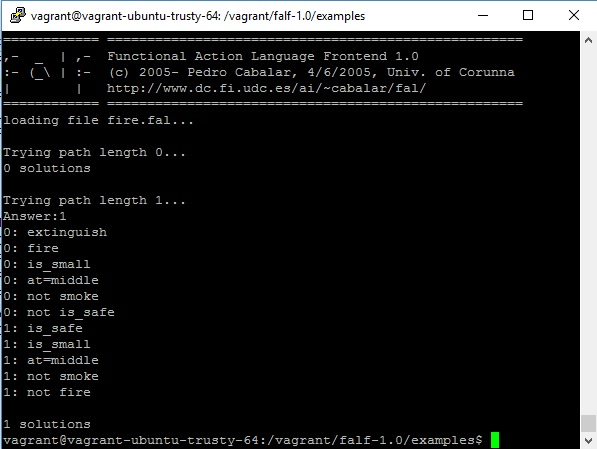
\includegraphics[scale=0.7]{capture_fire_small.jpg}



\chapter{Tool expressivity ($W_{10}$)}


In order to recreate a realistic scenario, key elements of the technical instrumentation provided were used:
\begin{enumerate}
\item {\color{Red}Instances} of two sorts: building and location were introduced.
\begin{verbatim}
instances

	building house, apartment, office.
	location door, window, middle, staircase, outside.

\end{verbatim}

\item {\color{Red} Fluents} are the type of functions whose values may vary along time, thus allowing the modelling of temporal problems.
 
To identify the fluents in the case of a fire scenario I have chosen specific attributes of the surrounding environment, that can have different values, corresponding to the different states the system could be in. 

A part of the fluents have boolean outcomes, thus meaning true/false, presence or absence of the specified element.

The fluents falling in this category are: 
{\it fire, smoke, is\_small, is\_safe, is\_door\_hot, is\_smoke\_under\_door, clothes\_on fire, standing, personnel\_alerted}.

Other fluents have values ranging in a given set (the instances declared): {\it at: location.  building\_type: building}.

\item 
{\color{Red} Default Values} are used with FAL to specify an initial value of a function. 
If none is specified, the value of the function is just {\it unknown}.
Examples of the usage of default values:
\begin{verbatim}
	fire: boolean = true.
	standing: boolean = true.
	personnel_alerted: boolean = false.
\end{verbatim}

\item Also, {\color {Red} inertia default} assumes that fluent values remain unchanged unless there exists evidence of the contrary.
This is enacted in the program automatically, as when we declare a FAL function as a fluent, we implicitly assert that it will behave under the inertia law.


\item {\color{Red} Actions} are functions that are implicitly generated, in order to transition from a previous state to a successor state.

The main actions identified in the case of a fire involve movement: {\it walk\_to, crawl\_to, descend\_staircase}, procedures that should be followed in certain conditions, for example, if one's clothes are on fire: {\it stop\_drop, roll}, or if the door is blocked: {\it escape\_window}.

 Another particular case, would be the usage of the extinguisher to put off a small fire, using the {\it extinguish} action.

Opening the door is another possible action : {\it open\_door}.

\begin{verbatim}
	walk_to: location.
	crawl_to: location.
	open_door: boolean=false.
	extinguish: boolean=false.
	escape_window: boolean=false.
	stop_drop, roll: boolean=false.
	descend_staircase: boolean=false.
\end{verbatim}

\item {\color{Red} Rules} along with the use of {\it functions} are the main components that define a problem. 
Herein, the rules included model the fluents and the events given.

\item A special type of rules, {\color{Red} constraints}, allow the pruning of undesired configurations, rejecting unwanted effects.
Constraints were used especially to control the use of actions, in order to specify when a certain action should not happen.

For instance, we do not want to open a door in case it is hot or smoke is coming from underneath it.
Also we cannot open it if we are not in front of it.

This can be illustrated as follows:
\begin{verbatim} 
	:- open_door, is_door_hot.
	:- open_door, is_smoke_under_door.
	:- open_door, at != door.
\end{verbatim}


\item The fire scenario created can be solved using the {\color {Red} planning} system provided by the FAL interpreter, that will try to obtain a {\it plan} (a sequence of actions) that allows going from the {\it initial} state to the {\it goal} state.

For example, initial conditions for a possible scenario, in which the fire is large, the entrance is not yet affected by flames, the location is the office where one works, and one's clothes caught fire,  would be:
\begin{verbatim}
initially

	smoke.
	at = middle.
	not is_small.
	not is_door_hot.
	not is_smoke_under_door.
	clothes_on_fire.
	building_type = office.
\end{verbatim}

Similarly, we need to specify the goal state:
\begin{verbatim}
goals
	is_safe.
\end{verbatim}


\item {\color{Red} Events} are non-inertial fluents, functions whose values may vary along the narrative but for which, in principle, there is no particular assumption relating its previous and successor value in any transition. 

This is why events can be used if the function may behave improperly in the case of a crash or an unexpected event, impeding the normal functioning of the system.

Events were used in this case to illustrate the sounding of the alarm, and calling the fire brigade:
\begin{verbatim}
events 

	call_fire_fighters: boolean=false.
	sound_alarm: boolean = false.
\end{verbatim}


\end{enumerate}


\chapter{Graph and experiments ($W_{11}$)}

 The code of the program, in its whole, can be viewed in Appendix ~\ref{app:original_code}.

Since we have declared default values for a part of the existing fluents:
\begin{verbatim}
fire: boolean = true.
is_safe: boolean = false.
standing: boolean = true.
personnel_alerted: boolean = false.
\end{verbatim}
the remainder will be the fluents whose values must be specified in the "initially" section of the code.
\begin{verbatim}
	smoke: boolean.
	at: location.
	building_type: building.
	is_small: boolean.
	is_door_hot: boolean.
	is_smoke_under_door: boolean.
	clothes_on_fire: boolean.
\end{verbatim}

The number of possible instance values for each of these last fluents are as follows: 
\begin{itemize}
\item[--] smoke: 2
\item[--] at: 4
\item[--] building\_type: 3
\item[--] is\_small: 2
\item[--] is\_door\_hot: 2
\item[--] is\_smoke\_under\_door: 2
\item[--] clothes\_on\_fire: 2
\end{itemize}
The total possible combinations of these fluents, in order to obtain an initial state, is:

$ 2 \times 4 \times 3 \times 2 \times 2 \times 2 \times 2 = 3 \times 2^7 = 384$.

Keeping this in mind, only a couple of possible, more realistic scenarios will be presented herein.

\section{Small home fire}

\begin{verbatim}
initially
   not smoke.
   at = middle.
   is_small.
   not is_door_hot.
   not is_smoke_under_door.
   not clothes_on_fire.
   building_type = house.
\end{verbatim}


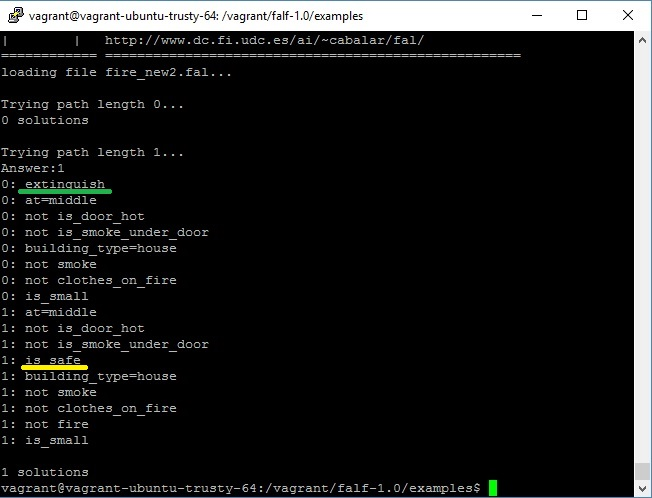
\includegraphics[scale=0.8]{Screenshot_small_home_fire.jpg}


As we can see, the FAL interpreter creates a plan, combining possible actions in a sequence, in order to transition between states.

Here, there is only one action that is enacted, {\it extinguish}, allowing the system to transition from state $0$ - where a small fire is present, to state $1$, where there is no fire.

Thus the system arrived in a safety state, accomplishing its goal and ceasing any further action.

\section{Large home fire}
\begin{verbatim}
initially
   smoke.
   at = middle.
   not is_small.
   not is_door_hot.
   not is_smoke_under_door.
   clothes_on_fire.
   building_type = house.
\end{verbatim}


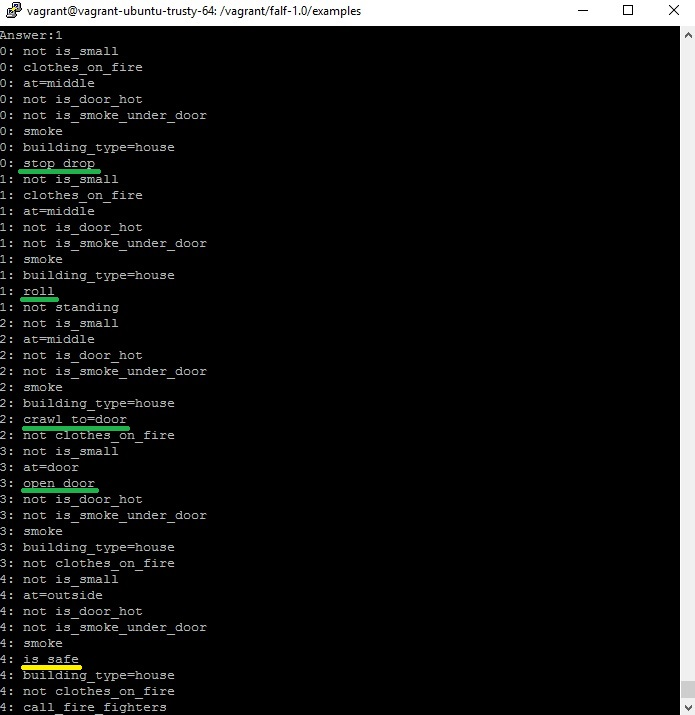
\includegraphics[scale=0.8]{Screenshot_home_fire.jpg}

The actions that transition between states are emphasised with a green line, whereas the desired final state is marked with yellow color.

As we can see, if one is caught in a home fire that is quickly spreading, before taking further actions, if one's clothes are on fire, this should be the first thing adressed.

The {\it stop, drop, roll} procedure is then enacted. The "at" fluent remains unchanged, because the location remains the same.

When the clothes are not on fire anymore, further action can be taken. 

In this case, because of the toxic smoke rising, the person will have to crawl to the nearest exit - the door. 

Once the door is open, the person is outside at safety and can call for specialised help.

The graph in figure ~\ref{fig:graph} outlines the flow of actions along the narrative.

\begin{figure}
\label{fig:graph}
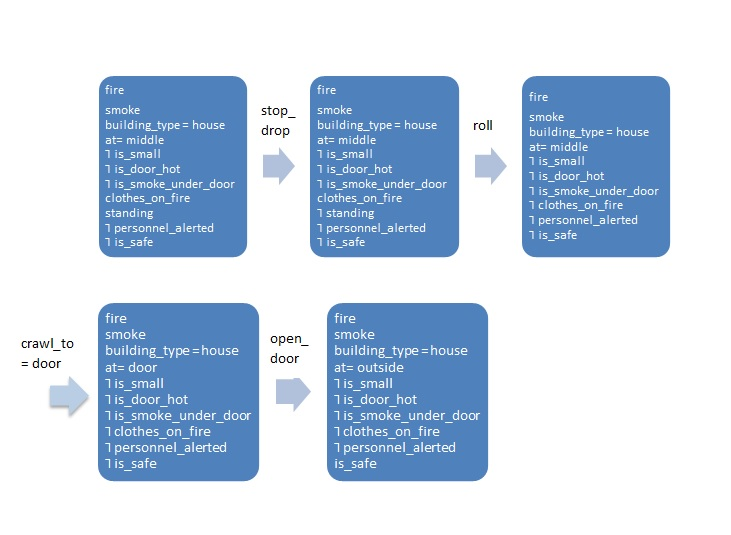
\includegraphics[scale=0.8]{Graph_home_fire.jpg}
\caption{Graph for large home fire scenario}
\end{figure}

\section{Apartment fire}
\begin{itemize}
\item Window escape
\begin{verbatim}
initially
   not smoke.
   at = middle.
   not is_small.
   not is_door_hot.
   is_smoke_under_door.
   not clothes_on_fire.
   building_type = apartment.
\end{verbatim}

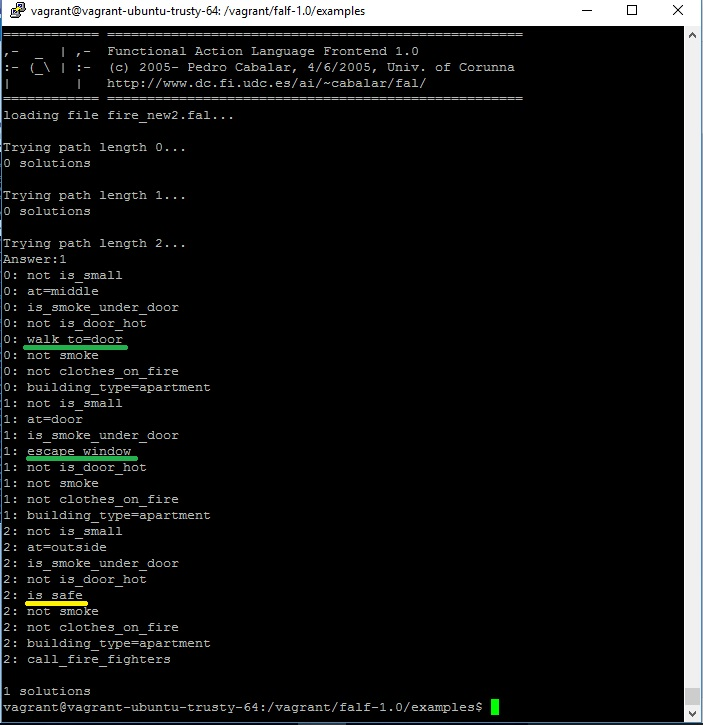
\includegraphics[scale=0.8]{Screenshot_ap_fire1.jpg}

In the case of a large apartment fire, if there isn't any smoke, one should walk to the nearest exit.

If the approached door seems to have smoke coming from underneath it, or if by testing with the back of one's hand, it feels warm/hot, it should not be openned.
This is because it might separate from even more fire. 

The person in cause is urged to exit using the window and then the fire escape stair.

\item Staircase escape

\begin{verbatim}
initially
   not smoke.
   at = middle.
   not is_small.
   not is_door_hot.
   not is_smoke_under_door.
   not clothes_on_fire.
   building_type = apartment.
\end{verbatim}


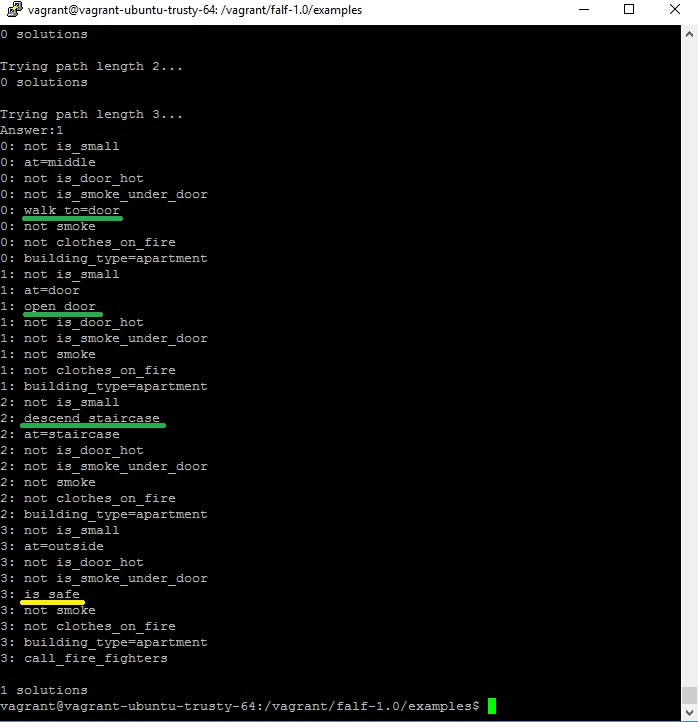
\includegraphics[scale=0.8]{Screenshot_ap_fire2.jpg}

If the door is not hot, one should slowly open it and pass through.

When arriving at the staircase, one should always use the stairs to descend, and not the elevator.

\end{itemize}

\section{Office fire}
\begin{verbatim}
initially
   smoke.
   at = middle.
   not is_small.
   not is_door_hot.
   not is_smoke_under_door.
   not clothes_on_fire.
   building_type = office.
\end{verbatim}

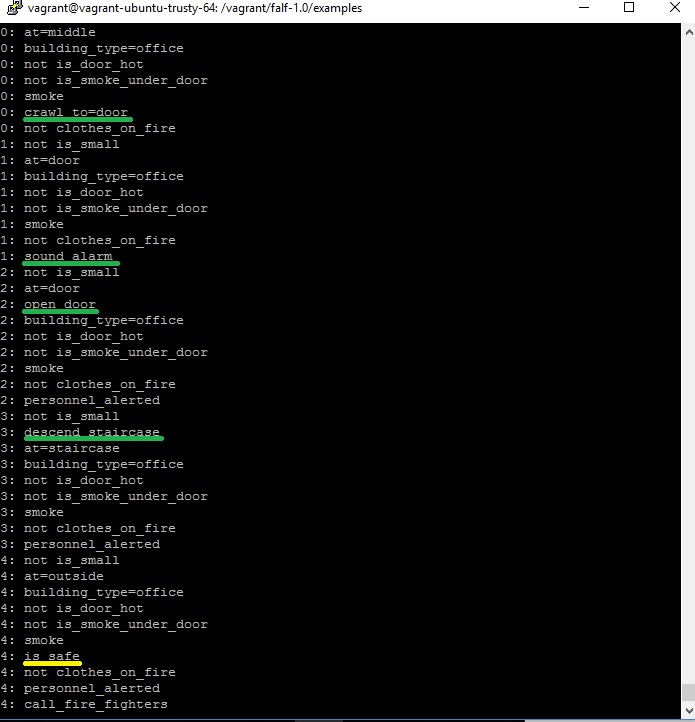
\includegraphics[scale=0.8]{Screenshot_office_fire.jpg}

In the case of an office fire, one must alert everyone else before leaving the building.
This is done by sounding the alarm, usually by pressing a button.

The rest of the procedures are similar to the previous examples.
The person uses the staircase instead of using an elevator, and stops doing anything else if the person's clothes are on fire, taking care of this issue first.

Last but not least, the person must alert the special forces, never assuming this has been done.



\chapter{Related Work and documentation ($W_{12}$)}

\section{Related approaches}

While scenario generation is of increasing concern, there is no generally accepted solution to it. Some of the existing prior approaches are enumerated bellow.

The paper \href{http://mariekepeeters.com/wp-content/uploads/2013/11/Ferdinandus-CSEDU2013-Automated-Scenario-Generation.pdf}{Automated Scenario Generation ~Coupling Planning Techniques with Smart Objects~}
  by Ferdinandus et al. (2013) introduces some previously tackled approaches of the subject, whilst simultaneously bringing forward an alternative solution, with their own program of scenario generation.

The following two works referenced refer to the creation of a game world that would reflect the desired learning task.
\begin{itemize}
\item[--] Martin et al.(2009) \cite{martin_2009} suggest creating an initial scenario centered around the training task. 
This is supposed to be extended with the addition of more events in order to increase the level of complexity. 
A shape grammar is then used to shape the requirements on the game world that follow from the resulting conceptual scenario.
\item[--] Lopes and Bidarra (2011) \cite{lopes_bidarra} focus on the creation of the scenario withing the virtual world, as well. 
They argue that the contents of the game world determine the trainee's experience.
Their proposal is that of using Smart Objects (Kallmann and Thalmann, 1998), which are annotated with the services they offer to their surroundings, such as the experiences they could offer a player.
These annotations can be used to steer the content selection process.
\end{itemize}

Some drawbacks to the presented alternatives would be the lack of explicit task representation, and the impossibility of deriving the expected action plan for the trainee.

\begin{itemize}
\item[--] Niehaus and Riedl (2009) \cite{niehaus_riedl} construct a scenario based on the trainee's expected action sequence, through the employment of automated planning techniques.
A default scenario plan is adapted so that the sequence of actions can be adjusted to fit the trainee's needs and abilities while maintaining a coherent storyline.
One of the most important advantage of this approach is the ability to track the actions a trainee is required to perform in order to accomplish the learning task.
\item[--] Grois et al. (1998) \cite{grois_1998} select events to persuade the trainee into performing the desired actions.
This is done by the employment of probabilistic networks, in order to compute specific events that are likely to create an opportunity to practise the learning task.
\item[--] Zook et al. (2012) \cite{zook_2012} make use of a basic set of events, using a genetic algorithm to extend, mutate and improve the sequence of events until an acceptable scenario has been generated.
\end{itemize}

The last two approaches offer interesting alternatives. 
Still, they are quite specific in their requirements of data, such as probability functions and quantitative scenario evaluation functions, that are all but trivial to define.


\section{Advantages and limitations of your solution}

{\it \textbf{ {\color {Blue} Possible strong points}}} of the current program could be:
\begin{itemize}
\item[--] The possibility of customizing the fire escaping scenario, depending on the type of the setting - house, apartment, office.
\item[--] The correct execution of the {\it stop-drop-roll } rule, in case one's clothes caught fire.
\item[--] The natural ordering of the actions, by importance. 
For instance, in case one's clothes are on fire, every other activity must be ceased, until the flames have been smothered.
\item[--] As it is crucial to reach a safe state before taking care of other aspects, such as calling the fire brigade, this is correctly emphasized.
\item[--] Prior to everything else, the "fight or flight" rule is accurately applied. 
This decision is important to be made as fast as possible, as fire can expand exponentially.
\item[--] The action of crawling is properly used in case of toxic smoke being present which can be fatal if inhaled.
\item[--] Alerting staff is correctly done before leaving the office building.
\end{itemize}

{\it \textbf{ {\color {Blue} There are a series of limitations }}} to my proposed solution:
\begin{itemize}
\item[--] The possibility of going through multiple rooms until reaching the final exit door is not yet modeled.
Currently, the person can only go to the door or to the window, supposing he is somewhere in the middle of the room.
\item[--] As it is, the program does not offer many solutions to escaping through other means than using the main entrance.
 If the door is not to be open, and there is no fire escape stair, the person should signal outside the window, while trying to call for help.
\item[--] Currently, the assumption is made that, if in an office, the alarm is placed near the door, while that is not the case in real life scenarios.

\end{itemize}

\section{Possible extensions of the current work}

The program could be extended in some of the following ways:
\begin{itemize}
\item A set of instructions on how to use a fire extinguisher could be introduced.
	\begin{enumerate}
	\item {\it pull pin}
	\item {\it aim at base of fire}
	\item {\it squeeze handle}
	\item {\it sweep from side to side}
	\end{enumerate}
\item There could be additional professional helping instruments, like a \textbf{fire blanket}, with specific instructions to follow, depending on the affected items:


\begin{tabular}{ | p{7cm} | p{7cm} | }
	\hline
	{\color{BurntOrange} \textbf{Substance}} & {\color{BurntOrange} \textbf{Person}} \\ 
	\hline
	 & \\
	Pull tape down until blanket is released 
		& Pull tape down until blanket is released \\
	 & \\
	Open blanket and fully and gently place over flames to seal fire from air 
		& Open blanket and fully wrap around the person to seal fire from air \\
	 & \\
	Turn off power supply. Leave blanket over fire. 
		& Seek medical assistance. \\
	 & \\
	\hline
\end{tabular}

\item A possible extension would be to determine the nature of the fire, in the case of a small fire.
Wheter it be a {\color{Brown} {\it chip pan}} fire, a {\color{Brown} {\it deep fat}} fire or a {\color{Brown} {\it waste bin}} fire, the nature of the type of fire is crucial in order to determine the type of instruments that should be used to extinguish it.

\item A \textbf{water extinguisher} could be introduced, keeping in mind that it should in no case be used on {\color{Brown} {\it electrical equipment}}, {\color{Brown} {\it flammable liquids}}, or {\color{Brown} {\it metal fires}}. 
It should only be used on {\color{Brown} {\it wood, paper}} and {\color{Brown} {\it textiles}}.

\item Another improvement would be the possibility of entering multiple rooms (as in real life) until reaching the exit of the apartment/ house/ office.

\item Extremely important, after leaving each of the visited rooms, one \underline{must} {\color{Red} \textit{\textbf{close the doors}}} behind one.
This is of the utmost importance as it would keep the fire from spreading.

\item If being traped in a room at a high level above ground, with no possibility of escaping through a window on a fire escape stair,
one could use a series of methods to ensure survival for as longer a period as possible, and to signal to outdoor rescuing forces:

\begin{itemize}
\item[--] wet towels should be placed underneath doors
\item[--] duct tape should be used to seal the means of ventilation
\item[--] windows should not be open
\item[--] if one desires to open a window, a wet sheet should be used to wrap around the window
\item[--] a colored piece of cloth should be used to hang outside the window, to signal to the special forces
\item[--] if one has ink, a message could be written on the cloth to be hung outside.
\end{itemize}

\item In the case of an office fire, one should use the {\it fire escape plan} to guide oneself out.
\end{itemize}




\chapter{Feedback ($W_{14}$)}

%The teaching objectives for this week are:

% \item To provide a constructive feedback on the strong/weak points of your performance during AI laboratory. This feedback focus on the scientific relevance of your results and it aims to complement the feedback encapsulated in the grade.

%\vspace{0.5cm}

\subsection{Self-assessment}

\begin{table}
\begin{tabular}{ll}
Aspect & Self-assessment\\ \hline
How did you manage to master the tool?& enthusiastic\\
How realistic was your scenario? & satisfactory\\
Relevance of the running experiments & satisfactory\\
Knowledge and skills achieved & enthusiastic\\ 
Capacity to market your effort and results through documentation and presentation& satisfactory\\
\hline
\end{tabular}
\caption{Self-assessment. Assess each aspect, with: enthusiastic, satisfactory, unsatisfactory, bad} 
\end{table}

%
{\color{Orange}‘What did you do well? Give examples’}
%
\begin{itemize}
\item[--] managed to accurately identify fluents: the attributes of the environment, that change with certain actions; 
e.g. : fire, smoke, at (location), is\_small, clothes\_on\_fire, etc.
\item[--] work with the use of constraints:
\begin{verbatim}
	:- open_door, is_door_hot.
	:- open_door, is_smoke_under_door.
	:- open_door, at != door.
	:- open_door, not personnel_alerted, building_type = office.

	:- walk_to = outside, not open_door. 
	:- walk_to = staircase, building_type = house.
	:- walk_to = staircase, not open_door.
\end{verbatim}
\item[--] modeling system behaviour by defining fluents at succesor states (primed values) based on predecessor states:
\begin{verbatim}
	personnel_alerted' :- sound_alarm.
	not fire' :- extinguish, fire.
	at' = outside :- escape_window.
	at' = outside :- descend_staircase.
	at' = outside :- open_door, building_type = house.
	at' = staircase :- open_door, building_type != house.
	not standing' :- stop_drop.
	not clothes_on_fire' :- roll, clothes_on_fire.	
\end{verbatim}
\item[--] correctly evidentiating between actions and events:

- in the case of {\it actions} there exists {\it  implicit value generation} at each transition

- in the case of {\it events} there is no particular assumption relating previous and successor values
\begin{verbatim}
actions
  walk_to: location.
  crawl_to: location.
  open_door: boolean=false.
  extinguish: boolean=false.
  escape_window: boolean=false.
  stop_drop, roll: boolean=false.
  descend_staircase: boolean=false.	

events 
  call_fire_fighters: boolean=false.
  sound_alarm: boolean = false.
\end{verbatim}

\end{itemize}
%
{\color{Orange}‘Where do you think the assignment is weak?’}
%
\begin{itemize}
\item[--] the tool $\rightarrow$ User Interface: information is hard to follow, unclear and not readable;
 hard to distinguish between transitions.
\item[--] the tool $\rightarrow$ for actions: have to define a lot of constraints, instead of giving rules;

(telling all the situations when an action CANNOT/MUST NOT be performed, instead of telling when an action CAN / MUST be performed)
\item[--] the information on the website could be better structured, maybe have a table of contents, in order to find specific information more easily.

\end{itemize}





\appendix

\chapter{Your original code}
\label{app:original_code}

\begin{verbatim}
instances

   building house, apartment, office.
   location door, middle, staircase, outside.


fluents

   fire: boolean = true.
   smoke: boolean.
   at: location.
   building_type: building.
   is_small: boolean.
   is_safe: boolean = false.
   is_door_hot: boolean.
   is_smoke_under_door: boolean.
   clothes_on_fire: boolean.
   standing: boolean = true.
   personnel_alerted: boolean = false.

	
actions

   walk_to: location.
   crawl_to: location.
   open_door: boolean=false.
   extinguish: boolean=false.
   escape_window: boolean=false.
   stop_drop, roll: boolean=false.
   descend_staircase: boolean=false.	
 
events 

   call_fire_fighters: boolean=false.
   sound_alarm: boolean = false.


rules	

   is_safe :- at = outside.
   is_safe :- at != outside, not fire.

   call_fire_fighters :- at = outside.

   sound_alarm :- not clothes_on_fire, building_type = office,
			                not personnel_alerted, at = door.
	
   personnel_alerted' :- sound_alarm.	
	
   :- not is_small, extinguish.
   :- clothes_on_fire, extinguish.
   not fire' :- extinguish, fire.
	
   at' = outside :- descend_staircase.
   :- descend_staircase, at != staircase.
   at' = staircase :- open_door, building_type != house.
	
   at' = outside :- open_door, building_type = house.
   :- open_door, is_door_hot.
   :- open_door, is_smoke_under_door.
   :- open_door, at != door.
   :- open_door, not personnel_alerted, building_type = office.
   
   at' = outside :- escape_window.
   :- escape_window, at != door.
   :- escape_window, at = door, not is_door_hot, not is_smoke_under_door.
   :- escape_window, building_type= office, not personnel_alerted.

   at' = walk_to.
   :- not unknown(walk_to), walk_to = at.
   :- not unknown(walk_to), smoke.
   :- not unknown(walk_to), clothes_on_fire.
   :- not unknown(walk_to), is_safe.
   :- not unknown(walk_to), is_small, fire.
   :- walk_to = outside, not open_door. 
   :- walk_to = staircase, building_type = house.
   :- walk_to = staircase, not open_door.
          
   at' = crawl_to.
   :- not unknown(crawl_to), crawl_to = at.
   :- not unknown(crawl_to), not smoke.
   :- not unknown(crawl_to), is_safe.
   :- not unknown(crawl_to), clothes_on_fire.
   :- not unknown(crawl_to), is_small, fire.
   :- crawl_to = outside, not open_door.
   :- crawl_to = staircase, building_type = house.
   :- crawl_to = staircase, not open_door.

   :- stop_drop, not clothes_on_fire.
   not standing' :- stop_drop.
   :- roll, standing.
        
   not clothes_on_fire' :- roll, clothes_on_fire.

   standing :- not clothes_on_fire.	


initially

   smoke.
   at = middle.
   not is_small.
   not is_door_hot.
   not is_smoke_under_door.
   clothes_on_fire.
   building_type = office.

goals

   is_safe.
	
	
\end{verbatim}



\bibliographystyle{plain}
\bibliography{is}


\vspace{2cm}
\begin{center}
Intelligent Systems Group\\

\includegraphics[width=10cm]{fig/footer}
\end{center}



\end{document}
